\chapter{Extending face tracks in MovieGraphs dataset}
\label{ch:char_track_extension}
The MovieGraphs dataset~\cite{moviegraphs} stands as a valuable dataset for understanding character emotions in movies, due to its rich annotations. However, upon close examination, it became apparent that the face tracks within the dataset faced challenges due to the limitations of face detection quality. Many instances revealed a frequent occurrence of missed character detections, leading to fragmented face tracks within a clip. Moreover, multiple track IDs were often assigned to the same character within a single shot, introducing complexities in tracking consistency. Furthermore, some shots lacked any face detections altogether, yet held untapped potential in offering a broader perspective on character emotions within a given scene.

Motivated by these observations and recognizing the need for enhanced character tracking precision, this chapter embarks on the task of extending face tracks within the MovieGraphs dataset~\cite{moviegraphs}. Our approach involves addressing the gaps in the ground-truth tracks within a shot, mitigating issues related to missed detections and multiple track IDs. Additionally, we aim to augment the dataset by incorporating shots with initially zero detections, unlocking valuable insights into character emotions in scenes that might have been overlooked.

The extension process unfolds in two key phases: first, we systematically recompute face detections and tracks for the movie scenes, aiming to improve the accuracy and continuity of character representation. Subsequently, a subset of the newly generated face tracks is assigned names based on their overlap with the original tracks present in the MovieGraphs dataset~\cite{moviegraphs}. To further enrich our understanding, we employ hierarchical clustering techniques to group all detections within a clip, allowing us to assign names to previously unnamed tracks based on the clustering results.

In essence, this chapter seeks to remedy the limitations of the existing face tracks in the MovieGraphs dataset~\cite{moviegraphs}, laying the groundwork for a more robust and comprehensive analysis of character emotions in cinematic narratives. By extending and refining face tracks, we aim to bridge gaps in character tracking consistency, providing a more accurate representation of the emotional journeys characters undertake throughout the unfolding scenes. Through these efforts, we strive to contribute to the nuanced exploration of emotions within the cinematic medium and offer an improved foundation for subsequent analyses in character-centric emotion recognition.

Fig.~\ref{fig:c1c_results} shows an example where original tracks did not have a single detection (due to the dark scene) for a scene in the ``Forrest Gump, 1994" movie, whereas our track-extension pipeline was able to correctly associate names to the unlabelled characters.

\begin{figure}[t]
\centering
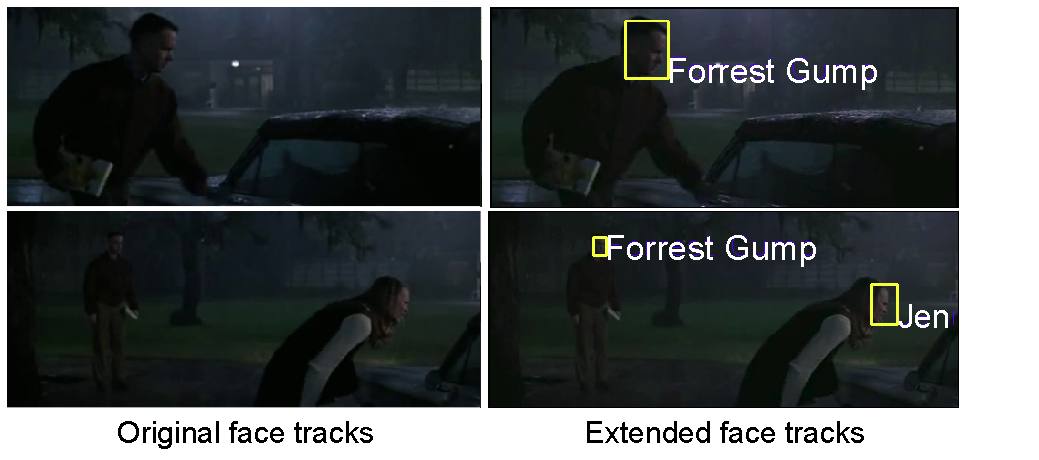
\includegraphics[width=0.80\linewidth]{Figures/c1c_results.pdf}
\vspace{-6mm}
\caption{Example face detections. The original face tracks do not work for dark scenes or profile faces, while our new detections and tracks are able to find them. Scene-036 from Forrest Gump, 1994.}
\vspace{-2mm}
\label{fig:c1c_results}
\end{figure}
